\chapter{Introduction}

The research work presented in this thesis has set ambitious goal to redesign the whole well established process of data management in finite element analysis software. It also proposes efficient methods to visualize finite element meshes and the results from complex finite element analyses.

Finite Element Analysis (FEA) is the term describing the entire process of modeling the physical system using the Finite Element Method (FEM). FEA consists of model generation, meshing, attribute assignment, solution, and post-processing. With the ongoing desire to solve more complex systems with better and better precision, an analysis has to process enormous amount of data in each of its phases. Traditional unstructured file-based representation of the mesh, input parameters, and the results from the solution is the bottleneck of the entire process. It lacks the scalability and complicates the development of the tools for engineers that are either preparing the input to FEM, or interpreting the output from FEM.

The solution of a large-scale finite element analysis itself can be parallelized and calculated in reasonable time on high-performance computing clusters. Nevertheless, in the end the results are transfered over a network and post-processed on an ordinary personal computer. Another concern is the colaboration and sharing of the model and the results between engineers and researchers. Limitations of the standard file-based approach lead to re-think the entire process of data management in FEA. The focus of the thesis is mainly on the post-processing of the results and the way the results are stored, transfered, and visualized. However, the storage format for the results introduced in the thesis was designed with the whole picture in mind and there is proposed a database-centric environment for complete FEA data management.

% Motivation example:
%The analysis of reactor vessels in nuclear power plants can serve as an motivation example (see Figure \ref{fig:motivation-example}). The analysis is used in the process of prolongation of the service life. The vessels are approximately 40 years old and detailed thermo-hydro-mechanical analysis has to be performed. Usually, two-dimensional axisymmetric or fully three-dimensional models are considered and it means hundreds of thousands degrees of freedom are used. The number of time steps is between 10,000 and 15,000. The output files contain displacements, strain and stress components, temperature, relative humidity (or moisture content) and several internal parameters (e.g., creep strains, damage parameter, etc.) in all time steps. The output files with size in the order of gigabytes are generated. More details can be found in \cite{Kruis2010,Krejci2015}.

% \begin{figure}[H]
% \centering
% 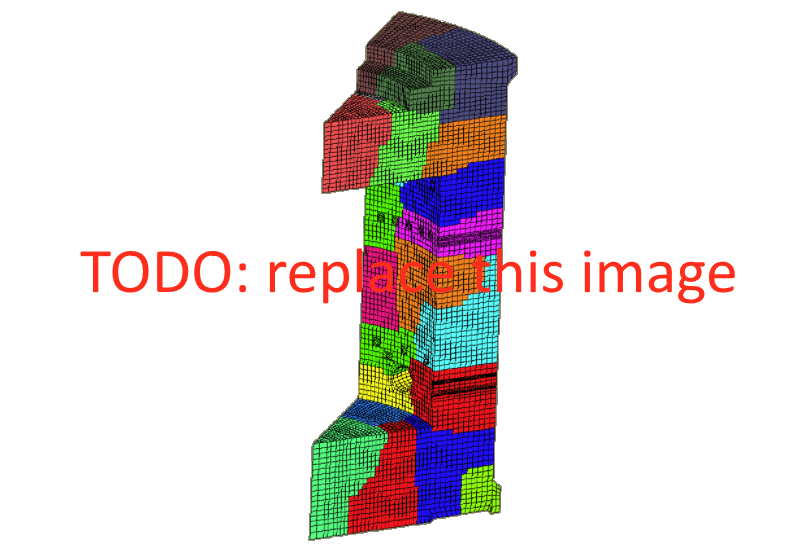
\includegraphics[width=0.5\textwidth]{figures/chapter-introduction/motivation-example}
% \decoRule
% \caption[Motivation example -- reactor vessel model visualization.]{Motivation example. Visualization of a nuclear power plant reactor vessel model, which is used to perform complex thermo-hydro-mechanical analysis.}
% \label{fig:motivation-example}
% \end{figure}


%The thesis is structured in the following manner. Chapter \ref{chapter:related-work} gives a brief revision of related work performed in FEA data management, file formats, data compression, and post-processing of the results from FEM. Chapter \ref{chapter:data-management} describes an alternative to file-based data management, proposes the new storage format for FEM results, and presents tools that are based on this new storage format. Sections \ref{sec:system-architecture} and \ref{sec:project-db-schema} contain a proposal of relational database model that connects all parts of the finite element analysis including geometry, model attributes, and simulation results, providing query interface and remote access over the Internet. Section \ref{sec:storage-format} contains detailed specification of the new data format. Section \ref{sec:postprocessing} presents the design of the post-processor that is built on top of the data management system. Section \ref{sec:implementation-details} summarizes technical details related to the implementation of the data management system and the post-processor.

%Chapter \ref{chapter:mesh-visualization} describes the implementation of efficient methods to visualize finite element meshes. Chapter \ref{chapter:approximation} presents a method for approximation of results from the finite element method using polynomial functions. Chapter \ref{chapter:SVD} proposes different approach to compress FEM results that is based on singular value decomposition. Each individual chapter contains its own section that evaluates the results of the proposed methods therein. Chapter \ref{chapter:conclusions} concludes the thesis with final remarks, benefits and weaknesses of the proposed solutions, and possible future work.

% TODO: describe content of the thesis

\section{Related work}

The contains a revision of related research work that deals with visualization of finite element meshes and results from FEM, file formats used for representation of FEM data, compression methods, and web-based FEA data management. A brief summary follows.


\subsection{Data compression and visualization}

The visualization of data produced by the finite element method is of two kinds. The discretization of the domain, called the finite element mesh, and the result fields that are mapped on the points inside the domain (either nodes or integration points). The general methods for visualization of 2D or 3D polygon (usually triangle) meshes have been researched in great depth. These data, when describing an object in great detail, can be relatively large in size if unoptimised. Therefore, many methods for reducing the size of data have been developed \cite{Alliez2005}. In \cite{Evans2014}, there is a wide survey of methods for data visualization and compression, especially with the focus on the web environment.

Progressive meshes represent one category of methods aiming for size reduction. They allow continuous, progressive coarsening or refinement of a polygonal mesh using a sequence of vertex-split operations. Progressive meshes were introduced originally in 1996 by Hoppe \cite{Hoppe1996} and their efficient implementation was presented in 1998 \cite{Hoppe1998}. Since then, there were various attempts to use Progressive meshes for compression and decompression of 3D meshes \cite{Gudukbay2002, Valette2004, Valette2009, Lavoue2013} and also for streaming of geometrical information from web server to client \cite{Alliez2001, Maglo2012}.

However, basic implementations of Progressive meshes and similar methods do not take into account vertex properties other than position. These methods are not designed to satisfactorily handle attributes assigned to mesh entities and their reconstruction. This is a major obstacle when applying the method to the data produced by FEM. Also, despite a considerable progress in the area of performance of Progressive meshes, decompression time is still a significant issue \cite{Limper2013}. In order to keep compression and decompression time within reasonable limits, an untolerable compromise must be made in compactness of the compressed representation.

% TODO: remove this paragraph?
A new way to visualize FEM data brings the isogeometric analysis introduced by Hughes \cite{Hughes2005}, which reuses the matematical representation of the input geometry created in CAD tools during the entire engineering process, including FEM analysis itself. In \cite{Stahl2017}, there is proposed an extension of this concept also for post-processing and visualization purposes.

Different approach for post-processing of FEM data can be to avoid trying to compress geometrical part (finite element mesh) and compress only result fields instead. The finite element mesh itself can be visualized using well-known methods of computer graphics and the result fields, as they can be viewed as a series of arbitrary rectangular matrices, can be handled separately by methods used for image compression. There are many image compression methods. The most commonly used are the discrete cosine transform \cite{Watson1994} used in JPEG standard and the wavelet transform used in JPEG 2000 standard \cite{Lui2001}.


\subsection{File formats}

There are many file formats that can be used for representation of input geometry of finite element software. In fact, McHenry in \cite{McHenry2008} presents about 140 file formats for representation of 3D models. On the other hand, there are very few open formats for representation of finite element meshes and results from the finite element method. Commercial software packages, such as Abaqus \cite{Abaqus}, use proprietary formats that are intended for internal use only or their documentation is not available. The available open formats are provided by open-source projects, e.g., Gmsh \cite{Geuzaine2009} or ParaView \cite{ParaView2005}, which are mainly used in academia. ParaView is based on the VTK file format \cite{VTK2015}. VTK can be considered as the only universal format for the representation of results from FEM that also supports data compression, eventhough the compression is based on ZIP method, which is not very suitable for FEM results. There is also not so widely used Gambit file format \cite{GAMBIT}, which supports representation of solution results.

GiD \cite{GiDWeb} is a pre and post processor for numerical simulations in science and engineering. Although it is a commercial software, its file format is documented \cite{GiDPostProcess} and accessible as the GiD is often connected to finite element software provided by other companies or organizations.


\subsection{Web-based data management}

Peng et al. in \cite{Peng2003} propose an implementation of an engineering data access system for a finite element analysis, which utilizes the Internet as the communication channel to access the analysis results. Besides the description of the overall architecture of the data management system and the communication between its components, the paper addresses three important aspects of any data management system: data storage scheme, data representation, and data retrieval. Although the exact type of database is not mentioned there, the relational type of database is expected to be used. Peng and Law in \cite{Peng2004} further build on the idea and present an Internet-enabled framework that allows users easy access to the FEA core service and the analysis results by using a web browser or other application programs.

The authors in \cite{Heber2007I} and \cite{Heber2007II} advocate for the use of a relational database management system in support of finite element analysis. They also propose a new way of thinking about data management in FEA as neither extreme data sizes nor integration (with other applications over the Web) was a design concern 40 years ago when the paradigm for FEA implementation first was formed. The papers also discuss how to make the transition from a file-based to a database-centric environment in support of large scale FEA.

Chen and Lin in \cite{Chen2008} present an Internet-based finite-element analysis framework, named Web-FEM, which allows users to access existing finite-element analysis service running on their machines from remote sites over the Internet. Weng in \cite{Weng2011} focuses on post-processing of FEA data using web technologies. The paper points out the fact that the Web is actually the only truly cross-platform environment. The implementation of the finite element simulation as cloud computing service is discussed in \cite{Ari2013}. The authors deal with the technical issues related to the design and implementation, as well as the issues related to the data privacy and security of the cloud services.

The benefits of web-based applications with respect to native desktop (or mobile) applications are summarized and explained in detail in \cite{Mouton2011} and \cite{Charland2011}. An example of remote rendering service for visualization of scientific data is ParaViewWeb \cite{Jourdain2011}. It is a JavaScript library that can be used to build applications with interactive 3D visualization inside the web browser. SimScale \cite{SimScale} is a commercial computer-aided engineering software product based on cloud computing that utilizes ParaViewWeb for the data visualization.

